\section{Conflict-serializability}

\begin{definition}[\textit{Conflict}]
    Two operations $o_i$ and $o_j$ ($i \neq j$) are in conflict if they address the same resource and at least one of them is write. 
    There are two possible cases: read-write conflicts or write-write conflicts.
\end{definition}
\begin{definition}[\textit{Conflict equivalent}]
    Two schedules are conflict-equivalent ($S_i \approx_C S_j$) if $S_i$ and $S_j$ contain the same operations and in all the conflicting pairs the transactions occur in the same order. 
\end{definition}    
\begin{definition}[\textit{Conflict serializable}]
    A schedule is conflict-serializable (CSR) if and only if it is conflict equivalent to a serial schedule of the same transactions. 
\end{definition}
\begin{property}
    VSR is a strict subset of CSR. 
\end{property}
\begin{proof}
    Consider the schedule $S = r_1(x) w_2(x) w_1(x) w_3(x)$, which is VSR but not CSR. 
    It can be verified that there is no conflict-equivalent serial schedule.
\end{proof}
\begin{property}
    CSR implies VSR.
\end{property}
\begin{proof}
    Assuming $S_1 \approx_C S_2$, we can prove that $S_1 \approx_V S_2$. 
    $S_1$ and $S_2$ must have: the same final writes (if not, there would be at least two writes in a different order, and since two writes are conflicting operations, the schedules would not be CSR), and the same reads-from relations (if not, there would be at least one pair of conflicting operations in a different order, and therefore $\approx_C$ would be violated).
\end{proof}

\paragraph*{Conflict graph}
To assess view-serializability, a conflict graph is constructed, with one node for each transaction $T_i$, and an arc from $T_i$ to $T_j$ if there exists at least one conflict between an operation $o_i$ of $T_i$ and an operation $o_j$ of $T_j$ such that $o_i$ precedes $o_j$.
\begin{theorem}
    A schedule is conflict-serializable if and only if its conflict graph is acyclic.
\end{theorem}
\begin{example}
    Consider the schedule 
    \[S: w_0(x) r_1(x) w_0(z) r_1(z) r_2(x) w_0(y) r_3(z) w_3(z) w_2(y) w_1(x) w_3(y)\]
    To test conflict serializability, follow these steps:
    \begin{enumerate}
        \item Create nodes based on the number of transactions in the schedule.
        \item Group operations based on the requested resource.
        \item Check all write-write and read-write relationships in each subset and add arcs accordingly. 
    \end{enumerate}
    For the given example, we obtain:
    \begin{itemize}
        \item $x: w_0 r_1 r_2 w_1$
        \item $y: w_0 w_2 w_3$
        \item $z: w_0 r_1 r_3 w_3$
    \end{itemize}
    \begin{figure}[H]
        \centering
        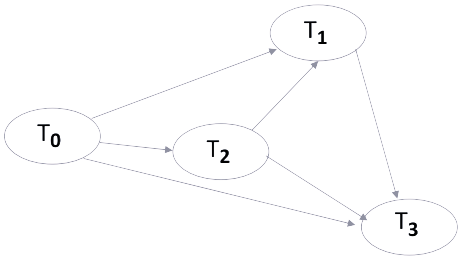
\includegraphics[width=0.25\linewidth]{images/conflict.png}
    \end{figure}
    Since there are no cycles in the graph, the schedule is conflict-serializable.
\end{example}
\begin{proof}
    We prove that CSR implies acyclicity. 
    Consider a schedule $S$ in CSR. 
    As such, it is $\approx_C$ to a serial schedule. 
    Without loss of generality we can label the transactions of $S$ to say that their order in the serial schedule is: $T_1 T_2 \dots T_n$.
    Since the serial schedule has all conflicting pairs in the same order as schedule $S$, in the conflict graph there can only be arcs $(i,j)$, with $i<j$. 
    Then the graph is acyclic, as a cycle requires at least an arc $(i,j)$ with $i>j$.
\end{proof}
\begin{proof}
    We prove that acyclicity implies CSR. 
    If $S$'s graph is acyclic then it induces a topological (partial) ordering on its nodes. 
    The same partial order exists on the transactions of $S$. 
    Any serial schedule whose transactions are ordered according to the partial order is conflict-equivalent to $S$, because for all conflicting pairs $(i,j)$ it is always $i<j$. 
\end{proof}